%%%%%%%%%%%%%%%%%%%%%%%%%%%%% Define Article %%%%%%%%%%%%%%%%%%%%%%%%%%%%%%%%%%
\documentclass{article}
%%%%%%%%%%%%%%%%%%%%%%%%%%%%%%%%%%%%%%%%%%%%%%%%%%%%%%%%%%%%%%%%%%%%%%%%%%%%%%%

%%%%%%%%%%%%%%%%%%%%%%%%%%%%% Using Packages %%%%%%%%%%%%%%%%%%%%%%%%%%%%%%%%%%
\usepackage{geometry}
\usepackage{graphicx}
\usepackage{caption}
\usepackage{subcaption}
\usepackage{amssymb}
\usepackage{amsmath}
\usepackage{amsthm}
\usepackage{empheq}
\usepackage{mdframed}
\usepackage{booktabs}
\usepackage{lipsum}
\usepackage{graphicx}
\usepackage{color}
\usepackage{psfrag}
\usepackage{pgfplots}
\usepackage{bm}
\usepackage{float}
\usepackage{physics}
\usepackage{hyperref}
\usepackage{xcolor}
\usepackage{titlesec}
\usepackage{algorithmic}
\hypersetup{
	colorlinks=true,
	linkcolor=blue,
	filecolor=magenta,
	urlcolor=cyan
}
\usepackage{animate}
\usepackage{svg}
% Quantum physics inner product
\newcommand{\innerp}[2]{\left\langle #1 \vert #2 \right\rangle}
\newcommand{\convolution}[2]{(#1 \star #2)}

%%%  \begin{figure}[htp]
%%%  	\centering
%%%  	\includegraphics[width=0.25\textwidth]{/path/to/image}
%%%  	\caption{}\label{fig:}
%%%  \end{figure}

% to write multiple lines of equations

%%  \begin{align*}
%%  \begin{split}
%%  	\ket{\phi} + \ket{\psi} &= \ket{\phi + \psi} \\
%%  	a \ket{\psi} &= \ket{a \psi}
%%  \end{split}
%%  \end{align*}

\newcommand{\e}[1]{\times 10^{#1}}

\usepackage{listings}
\lstset{showstringspaces=false} % pretty embeded code in LaTeX
%%%%%%%%%%%%%%%%%%%%%%%%%%%%%%%%%%%%%%%%%%%%%%%%%%%%%%%%%%%%%%%%%%%%%%%%%%%%%%%

% Other Settings

%%%%%%%%%%%%%%%%%%%%%%%%%% Page Setting %%%%%%%%%%%%%%%%%%%%%%%%%%%%%%%%%%%%%%%
\geometry{a4paper}

%%%%%%%%%%%%%%%%%%%%%%%%%% Define some useful colors %%%%%%%%%%%%%%%%%%%%%%%%%%
\definecolor{ocre}{RGB}{243,102,25}
\definecolor{mygray}{RGB}{243,243,244}
\definecolor{deepGreen}{RGB}{26,111,0}
\definecolor{shallowGreen}{RGB}{235,255,255}
\definecolor{deepBlue}{RGB}{61,124,222}
\definecolor{shallowBlue}{RGB}{235,249,255}
%%%%%%%%%%%%%%%%%%%%%%%%%%%%%%%%%%%%%%%%%%%%%%%%%%%%%%%%%%%%%%%%%%%%%%%%%%%%%%%

%%%%%%%%%%%%%%%%%%%%%%%%%% Define an orangebox command %%%%%%%%%%%%%%%%%%%%%%%%
\newcommand\orangebox[1]{\fcolorbox{ocre}{mygray}{\hspace{1em}#1\hspace{1em}}}
%%%%%%%%%%%%%%%%%%%%%%%%%%%%%%%%%%%%%%%%%%%%%%%%%%%%%%%%%%%%%%%%%%%%%%%%%%%%%%%

%%%%%%%%%%%%%%%%%%%%%%%%%%%% English Environments %%%%%%%%%%%%%%%%%%%%%%%%%%%%%
\newtheoremstyle{mytheoremstyle}{3pt}{3pt}{\normalfont}{0cm}{\rmfamily\bfseries}{}{1em}{{\color{black}\thmname{#1}~\thmnumber{#2}}\thmnote{\,--\,#3}}
\newtheoremstyle{myproblemstyle}{3pt}{3pt}{\normalfont}{0cm}{\rmfamily\bfseries}{}{1em}{{\color{black}\thmname{#1}~\thmnumber{#2}}\thmnote{\,--\,#3}}
\theoremstyle{mytheoremstyle}
\newmdtheoremenv[linewidth=1pt,backgroundcolor=shallowGreen,linecolor=deepGreen,leftmargin=0pt,innerleftmargin=20pt,innerrightmargin=20pt,]{theorem}{Theorem}[section]
\theoremstyle{mytheoremstyle}
\newmdtheoremenv[linewidth=1pt,backgroundcolor=shallowBlue,linecolor=deepBlue,leftmargin=0pt,innerleftmargin=20pt,innerrightmargin=20pt,]{definition}{Definition}[section]
\theoremstyle{myproblemstyle}
\newmdtheoremenv[linecolor=black,leftmargin=0pt,innerleftmargin=10pt,innerrightmargin=10pt,]{problem}{Problem}[section]
%%%%%%%%%%%%%%%%%%%%%%%%%%%%%%%%%%%%%%%%%%%%%%%%%%%%%%%%%%%%%%%%%%%%%%%%%%%%%%%

%%%%%%%%%%%%%%%%%%%%%%%%%%%%%%% Plotting Settings %%%%%%%%%%%%%%%%%%%%%%%%%%%%%
\usepgfplotslibrary{colorbrewer}
\pgfplotsset{width=8cm,compat=1.9}
%%%%%%%%%%%%%%%%%%%%%%%%%%%%%%%%%%%%%%%%%%%%%%%%%%%%%%%%%%%%%%%%%%%%%%%%%%%%%%%

%% Centering section titles
\titleformat{\section}[block]{\Large\bfseries\filcenter}{}{1em}{}

%% norm
%%\newcommand\norm[1]{\lVert #1 \rVert}


\title{Machine learning - random}
\author{Aheer Srabon}
\date{}

\begin{document}
\maketitle

\section{Section 1}
% Using TensorFlow keras
\begin{lstlisting}[language=Python]
from tensorflow import keras
from tensorflow.keras import layers

# Create a network with 1 linear unit
model = keras.Sequential([
	layers.Dense(units=1, input_shape=[3])
])
\end{lstlisting}

\noindent keras\.Sequential creates a neural network as a stack
of layers. The above example defines a model accepting three input
features and producing a single output. The first argument units
define how many outputs we want. The second argument input\_shape
tells keras the dimensions of the input. input\_shape is the number
of columns of the DataFrame except for the output column. It is a
python list to permit use of more complex datasets.

\noindent Neural networks typically organize their neurons into layers.
When we collect together linear units having a common set of inputs, we
get a \textbf{dense} layer.

\begin{figure}[htp]
	\centering
	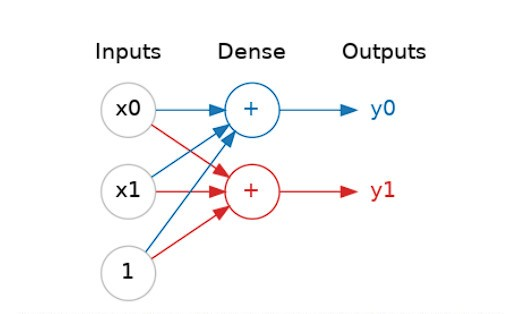
\includegraphics[width=0.5\textwidth]{../assets/machine_learning_random/denser_layer_with_two_inputs_and_a_bias.jpg}
	\caption{A dense layer of two linear units receiving two inputs and a bais.}
\end{figure}

\noindent Each layer in neural network performs some kind of relatively
simple transformation. Through a deep stack of layers, a neural network can
transform its inputs in more and more complex ways. In a well-trained
neural network, each layer is a transformation getting us a little bit
closer to a solution. A "layer" in Keras is a very general kind of thing.
A layer can be, essentially, any kind of data transformation (like
convolution, recurrence). 

\subsection{The activation function}
\noindent It turns out that two dense layers with nothing in between
are no better than a single dense layer by itself. Dense layers by
themselves can never move us out of the world of lines and planes. 
An activation function brings non-linearity to the model. An 
\textbf{activation function} is simply some function that is applied to
each of a layer's outputs (its activations). The most common is the
rectifier function $ max(0,x) $. When a attach a rectifier to a linear
unit, we get a rectified linear unit or \textbf{ReLU}. Applying a ReLU
activation to a linear unit means the output becomes $ max(0, wx + b) $,
which might be drawn like:

\begin{figure}[htp]
	\centering
	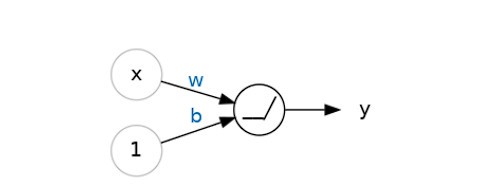
\includegraphics[width=0.5\textwidth]{../assets/machine_learning_random/rectified_linear_unit.jpg}
	\caption{A rectified linear unit.}
\end{figure}

\noindent Stacking dense layers,

\begin{figure}[htp]
	\centering
	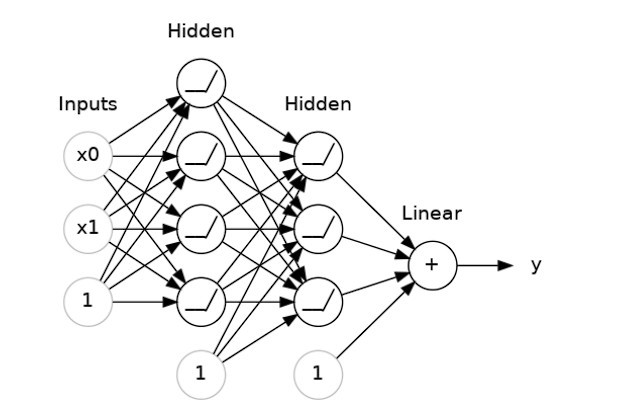
\includegraphics[width=0.5\textwidth]{../assets/machine_learning_random/stack_of_dense_layers.jpg}
	\caption{A stack of dense layers makes a "fully-connected" network.}
\end{figure}

\noindent The final (output) layer is a linear unit (with no activation function).
That makes this network appropriate to a \emph{regression}, task. Other tasks (like
classification) might require an activation function on the output.

\subsection{Building sequential models}
The Sequential model we've been using will connect together a list of layers
in order from first to last: the first layer gets the input, the last layer
produces the output. This creates the model in the figure above:

\begin{lstlisting}[language=Python]
from tensorflow import keras
from tensorflow.keras import layers

model = keras.Sequential([
    # the hidden ReLU layers
    layers.Dense(units=4, activation='relu', input_shape=[2]),
    layers.Dense(units=3, activation='relu'),
    # the linear output layer 
    layers.Dense(units=1),
])
\end{lstlisting}

\noindent Sequential takes a list of layers. Sometimes, some other
layer are put between the Dense layer and its activation function. In
these cases, the activation can be defined on its own Activation layer.

\begin{lstlisting}[language=Python]
from tensorflow import keras
from tensorflow.keras import layers

model = keras.Sequential([
    # the hidden ReLU layers
    layers.Dense(units=4, activation='relu', input_shape=[2]),
    layers.Dense(units=3)
    # The activation is in its own layer. Between
    # the Dense layer and the Activation layer, some other layers can be 
    # put
    layers.Activation('relu')
    # the linear output layer 
    layers.Dense(units=1),
])
\end{lstlisting}

\noindent To train a neural network, the following things are needed,
\begin{itemize}
	\item The model iteself
	\item Training data
	\item A loss function (tells the network what problem to solve)
	\item An optimizer (tells the network how to solve the problem)
\end{itemize}

\noindent Some example of loss functions are,
\begin{itemize}
	\item Mean Absolute Error (MAE)
	\item Mean Squared Error (MSE)
	\item Huber loss
\end{itemize}

\subsection{Stochastic gradient descent}
\noindent Virtually all of the optimization algorithms used in deep learning
belong to a family called \textbf{stochastic gradient descent}. They are
iterative algorithms that train a network in steps.
\begin{enumerate}
	\item Sample some training data and run it through the network to make
		predictions
	\item Measure the loss between the predictions and the true values
	\item Finally, adjust the weights in a direction that makes the loss smaller
\end{enumerate}

\noindent Repeat the above process until the loss as small as necessary (or until
it won't decrease any further). Each iteration's sample of training data is called
a minibatch (or often just "batch"), while a complete round of the training data
is called an epoch. The number of epochs you train for is how many times the
network will see each training example.

\begin{figure}[htp]
	\centering
	\includemovie{2cm}{2cm}{../assets/machine_learning_random/stochastic_gradient_descent.gif}
	\caption{Training a neural network with stochastic gradient descent}
\end{figure}
\end{document}
